% Test fixture: a grouped bar chart in pgfplots' default style (Computer Modern, boxed axes, legend box,
% default colour cycle). Input for the "unify three existing figures" task; the data must survive unchanged.
\documentclass[border=2pt]{standalone}
\usepackage{pgfplots}
\pgfplotsset{compat=1.18}
\begin{document}
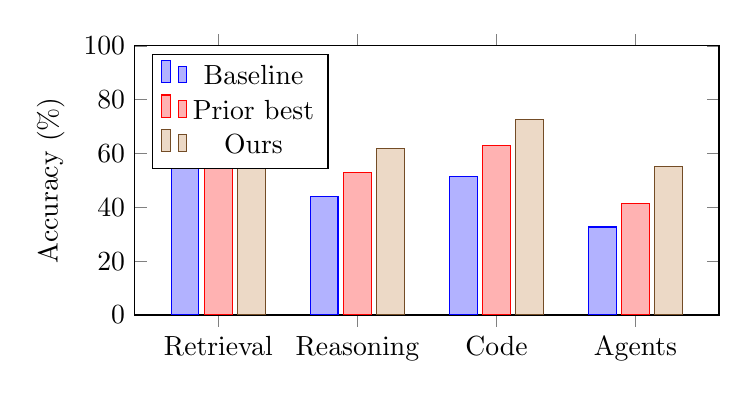
\begin{tikzpicture}
\begin{axis}[ybar, width=9cm, height=5cm, ymin=0, ymax=100, ylabel={Accuracy (\%)},
  symbolic x coords={Retrieval, Reasoning, Code, Agents}, xtick=data, legend pos=north west, enlarge x limits=0.2]
\addplot coordinates {(Retrieval,58.2) (Reasoning,44.1) (Code,51.3) (Agents,32.7)};
\addplot coordinates {(Retrieval,66.4) (Reasoning,52.8) (Code,63.0) (Agents,41.5)};
\addplot coordinates {(Retrieval,74.1) (Reasoning,61.7) (Code,72.5) (Agents,55.2)};
\legend{Baseline, Prior best, Ours}
\end{axis}
\end{tikzpicture}
\end{document}
